\documentclass[]{ecca}
\usepackage[T1]{fontenc}
\usepackage[latin1]{inputenc}
\usepackage{indentfirst}
\usepackage{longtable}
\usepackage{xcolor,graphicx}
\usepackage{float}
\graphicspath{ {./Graphics/} }
\usepackage{hyperref}
\hypersetup{%
   colorlinks = {true},
   urlcolor = {blue},
   linkcolor = {black},
   citecolor = {black},
   pdfauthor = {Quinn Batten},
   pdftitle = {Comprehensive Project},
   pdfkeywords = {Unemployment, Self-employment, Entrepreneurship, VAR, Vector Autoregression}
}

\usepackage{multido}

\title{Unemployment and Entrepreneurship in the US Economy}
\author{Quinn Batten}

\begin{document}

\maketitle

\begin{abstract}

I use a large dataset, VAR modeling techniques, and a detailed model selection procedure to investigate the relationship between unemployment and entrepreneurial activity in the US. I find that these variables are useful predictors of each other and that a shock to self-employment likely increases unemployment in the short-term and decreases it in the long-term. This has important implications for the use of entrepreneurial activity as a policy lever.

\end{abstract}

\section*{Introduction}
Soon after the Great Recession, the executive branch of the U.S. government moved to implement programs that encouraged entrepreneurship, in the hopes that increased entrepreneurship would help the recovery (The White House, 2016). However, that may have been a misinformed policy choice. The literature suggests that a shock to entrepreneurship causes an increase in unemployment starting within roughly six months of the shock and continuing for five to fourteen years after the shock. There should also be a long-term decrease in unemployment, but there is little information about the expected timing of the response of unemployment to a shock in entrepreneurship in the U.S.; without that information, it's hard to determine what the best policy choice is. Given that the U.S. government has decided to use entrepreneurship as a policy response to recessions, we must ensure that they have the information they need in order to do so effectively. This paper aims to investigate this question in detail and provide an assessment of the U.S. economy's behavior with regard to this relationship, in hopes of providing support for policy makers. 

There are several aspects of this paper that will add value to the literature: the dataset used spans an unusually long time range, the model type is especially suitable to this research question, and focusing on the US allows for policy recommendations tailored to the US economy. As far as I am aware, my data set is unique in its length and granularity, and has not been used in any major papers so far. The broad time range covered provides greater statistical sensitivity; it also means the results are more robust to the changing features of the US economy and therefore are more generalizable. In terms of statistical techniques, I use a vector autoregression (VAR), which is a type of model that allows for bidirectional causation in time series data.

I find that both variables Granger-cause each other. That is, they are useful in predicting each other. I also find that a positive shock to self-employment has a short-term positive and long-term negative effect on unemployment. Secondary findings uncovered during my model selection process provide further insight into the relationship between the variables of interest and offer interesting directions for future research. My results are mostly consistent with my hypotheses and the findings of the field, and they provide a sense of the timeline of these effects in the US, which few previous studies have done.

\section{Literature Review}

The relationship between entrepreneurship and unemployment is complex, and for many years, researchers have struggled to create a satisfactory model \citep{geroski95}. There are several difficulties in modeling this relationship, one of which is that there seems to be bidirectional causation with small and immediate effects. Vector autoregression (VAR) is useful for this research question because it is able to account for bidirectional causality in and unidirectional within-period effects in time-series data. I will address the causal directions separately from each other.

\subsection{Entrepreneurship's Effect on Unemployment}

Evidence indicates that a rise in entrepreneurship causes a short-term decrease in unemployment, followed by a medium-term increase, and then a decrease in the long-term. The short- and medium-term effects have weaker evidence behind them, and it is not certain that they exist at all. There is not a consensus about the long-term effect, but there is strong evidence for it.

In the very short term, there seems to be a drop in unemployment when entrepreneurial activity increases. This makes theoretical sense: when a new firm is created, new employees are hired, and some of those hires may be drawn from the pool of unemployed people \citep{fritsch04, pfeiffer00}. Further, smaller firms grow faster than larger firms, so, ceteris paribus, a temporary shift in industry structure towards small firms should mean an increased rate of employment growth \citep{evans87, audretsch01}. The specification of my final model does not allow me to test this hypothesis; my data is aggregated to half-yearly periods, which is too long to capture this effect alone.

In the short- and medium-term, some papers have found a positive effect on unemployment, lasting from one to six years \citep{fritsch04, dejardin11, baptista07}. \citeauthor{fritsch04} proposed that this occurs because entrants crowd out incumbents very quickly after founding, causing incumbents to exit, but newcomers don't expand their own employment until later years. However, some studies have not found this effect \citep{audretsch01}.

In the long-term, it is likely that entrepreneurship decreases unemployment due to increased innovation, increased competition, and other factors. There is fairly strong support for this effect in the literature \citep{plehn12, matejovsky14, fritsch04, dejardin11, audretsch98, koellinger09, thurik08}. One hypothesized mechanism for this is that entrepreneurship drives economic growth. Increased growth, in turn tends to push unemployment down towards its structural level \citep{matejovsky14}. Entry also increases competition, thereby reducing the market power of current participants, increasing total market output, and increasing labor input \citep{audretsch01}. In a review of seven papers, the lag between increased entrepreneurship and the long-term reduction in unemployment taking effect varied in length from six to fourteen years \citep{plehn12}. 

%**Audretsch said short lags(4yrs) do not pick up the effect of self-emp decreasing unemp in long-term
%**Matejovksy 2014 p618 says self-emp is a sector of distress? making it even weirder that I didn't pick up on that short-term effect
%**Matejovsky has used self-emp rate like I did as a measrue of entrepreneurship (p617).

\subsection{Unemployment's Effect on Entrepreneurship}

The balance of evidence indicates that unemployment causes an increase in entrepreneurial activity. Most of the literature on this question builds on Knight's model of employment, which focuses on the individual's choice between regular employment, entrepreneurship, and leaving the labor market. In this model, there is a push effect towards entrepreneurship from unemployment, and a pull effect towards unemployment when there is high growth in the economy. There is a push effect from unemployment because increased unemployment means decreased likelihood of successfully finding a job, and therefore decreases the expected opportunity cost of entrepreneurship--- this will be further discussed in the Theory section. Growth is important here as well, and it complicates the picture. When growth is rapid, the expected returns from entrepreneurship are higher; when growth is slow, entrepreneurship is unlikely to be rewarding. New businesses have a high failure risk in any situation, and the increased risk of failure that comes with starting a business in a slow economy deters the risk-averse (Geroski 1995). Several papers have found that unemployment increases entrepreneurship (Matejovsky 2014, Plehn, Audretsch 1998 \& 2001, Baptista 2007). Papers that do not control for growth may be less sensitive to this effect, since high unemployment is associated with slow growth, which decreases the pull effect of entrepreneurship. However, the role of growth in this relationship is contentious, and it may not have the significant effects that some aspects of theory suggest.  Unemployment's effect on entrepreneurship may be a U-shaped relationship, where moderate unemployment drives increased entrepreneurship through the push effect, while high unemployment decreases it through a weakening of the pull effect \citep{berglann11}. 

\subsection{Defining and Measuring "Entrepreneurship"}

This relationship is complicated considerably by the difficulty of defining and measuring "entrepreneurship." There are two widely used meanings of the word "entrepreneur." Firstly, it can mean someone who runs their own business; this category is defined by things like taking on a share of risk, being self-employed, and running a small business. Secondly, it can mean a Schumpeterian entrepreneur: someone who brings an innovative idea to market. Schumpeterian entrepreneurs are quite different from a typical franchise-owner, bodega-owner, therapist, plumber, etc; they come in many shapes and sizes---  Henry Ford, Walt Disney, and Russell Simmons are all famous Schumpeterian entrepreneurs. It is exceedingly difficult to measure Schumpeterian entrepreneurship, since it appears in many organizational structures and sizes, and there is no common behavior or measurable feature by which to identify this type of entrant. Most papers measure "entrepreneurship" by using some variation on firm entry, firm churn, or self-employment. These measures capture the first sense of entrepreneur but not the second. Further, even disregarding the division I've just drawn, there are also many different categories of entrants--- in a purely structural or legal sense--- each of which has unique effects and expected behaviors. Storey's 1991 paper divides firms into "wholly new firms," "self-employed," and "entrants" (the last of which also has three subcategories). Storey finds that these categories are statistically and practically meaningful in several ways. For example, people who turn to entrepreneurship because of recent unemployment have a lower success rate than other entrepreneurs (Berglann 2011). However, most papers ignore this heterogeneity, choose one of the more common measures, and describe their results as being representative of "entrepreneurship" as a whole. It is vital to take into account the heterogeneity of entrepreneurship, because it really isn't a suitably precise category on its own. This imprecision is responsible for a significant amount confusion and conflicting results in the literature. See Audretsch' 2001 paper for evidence of this. Audretsch mentions some of the conflicts partially caused by imprecision and points vaguely to imprecise definition of terms as a cause, but does not fully discuss and describe the extent of the problem. 

In my paper, I use self-employment as a measure of entrepreneurship. This measure captures a small subset of entrepreneurs, and the results can only be generalized to that subset. Some differences we expect to between the self-employed and other types of entrepreneur: this subset of entrepreneurs is more likely to have turned to entrepreneurship as a way of avoiding unemployment, and their firms tend to have less growth potential than other types of entrepreneur \citep{berglann11, gries09}.


\section{Data}

I use two variables, self-employment rate and unemployment rate. Unemployment rate was available directly, but I had to construct the self-employment rate variable by dividing self-employment level by total employment level. Self-employment rate is well-established as a measure of entrepreneurship \citep{matejovsky14}. All data is national for the United States and was acquired at a monthly frequency. The range is January 1948 to June 2016. All variables were acquired from the Bureau of Labor Statistics (BLS). The variable names, or "serial names," which can be used on the BLS website, bls.gov, to acquire these specific data sets, are LNU02027714 for self-employment level (in thousands of people), LNU02000000 for total employment level (in thousands of people), and LNU04000000 for unemployment rate. For the final model, all data has been converted to a biannual (twice yearly) frequency by finding the mean of all months within each half-year period. All variables were log-transformed for the final model. The rationale for that decision will be discussed further in the Results section. There were no missing values for any of the variables, and all variables were unadjusted; seasonally-adjusted variables can cause serious problems with VARs and other models (L�tkepohl, 63). See Table \ref{sumstat1}, below, for summary statistics for the untransformed variables and Table \ref{sumstat2} for the transformed variables. Figures 1 and 2 show the untransformed variables over time.

\begin{center}
	$H_0$: IRF(1) = 0;  $H_A$ IRF(1) $\neq$ 0 \\
	t-statistic = $\frac{\hat{x}}{SE(x)} =\frac{0.001094}{0.001272}=0.860$ \\ 
\end{center}


\begin{table}[!h]
	\centering
	\caption{Summary Statistics for untransformed variables}
	\label{sumstat1}
	\begin{tabular}{lllll}
		\hline 
		Variable	& Mean &	St. Dev. & Min & Max \\
		\hline
		Unemployment rate & 5.811	&	1.644 &	2.750 & 10.583  \\
		Self-employment level &	9262.086	& 1088.879 &	6978.83	& 10878.8 \\
		Self-employment  rate & 0.0991619 &	0.0329 &	0.0628	& 115.836  \\
		\hline 
	\end{tabular}
\end{table}



\begin{table}[!h]
	\centering
	\caption{Summary Statistics for natural-logged variables, as used in final model}
	\label{sumstat2}
	\begin{tabular}{lllll}
		\hline
Variable            & Mean   & St. Dev. & Min    & Max            \\
\hline
Unemployment rate    & 1.720  & 0.284  & 1.012     & 2.359 \\
Self-employment rate & -2.358 & 0.296    & -2.767 & -1.672 \\
\hline
	\end{tabular}
\end{table}

\begin{figure}[!h]
	\centering
	\fbox{\parbox{\textwidth}{\centering
			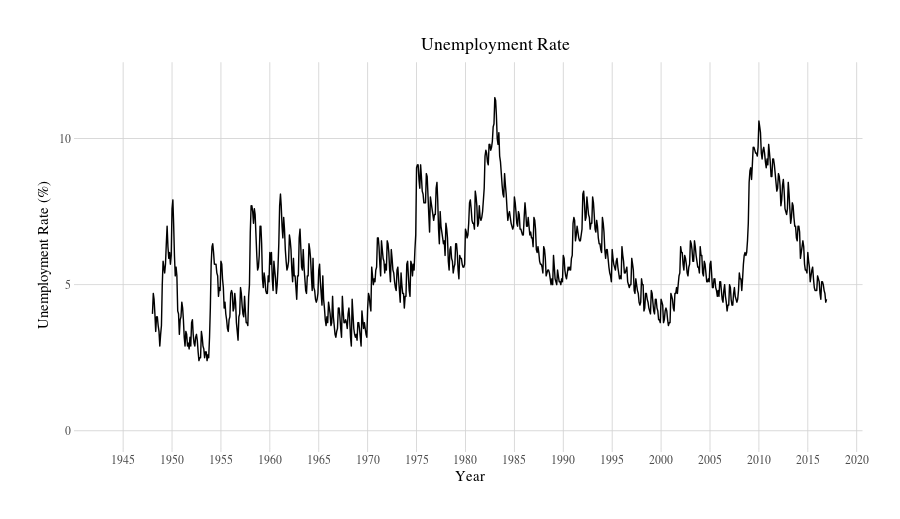
\includegraphics[width=\linewidth]{Unemp}
	}}
	\medskip\\
	\caption{Unemployment Rate in the U.S. Monthly, 1948-2016, Untransformed}
	\label{fig:data1}
\end{figure}
\begin{figure}[!h]
	\centering
	\fbox{\parbox{\textwidth}{\centering
			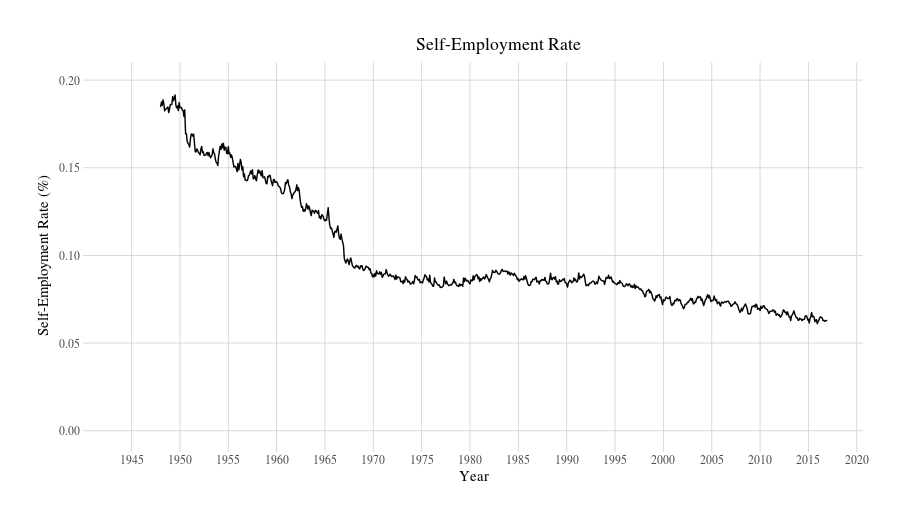
\includegraphics[width=\linewidth]{Selfemp}
	}}
	\medskip\\
	\caption{Self-Employment Rate in the U.S. Monthly, 1948-2016, Untransformed}
	\label{fig:data2}
\end{figure}
\textit{}

\section{Theory}

This paper rests on two bodies of theory. One is \citeauthor{knight}'s model of employment, where an individual weighs the relative expected utilities of employment and entrepreneurship (1921, pg. 273). My hypothesis about the behavior of self-employment in response to changes in the unemployment rate is derived from this theory. The second body of theory I draw from is Schumpeterian growth theory, the relevant aspect of which is the expectation that increasing firm churn is associated with innovation and therefore growth. It is a fairly straightforward extension of this theory to expect that employment will also expand in response to increased firm entry and innovation \citep{fritsch04}. My hypotheses are based on these two bodies of theory as well as the empirical evidence discussed in the literature review.

\subsection{Unemployment's Effect on Self-Employment}

I hypothesize that an increase in unemployment will cause an increase in self-employment. I'll expand on the hypothesized mechanism. An increase in unemployment will affect all those who are not currently employed, both the unemployed and those who are newly entering the labor market, and perhaps a small subset of those who are employed--- we'll call these groups "relevant entrants." The unemployed are relevant entrants, because they are (by definition) currently engaged in a job search, but are able to switch to an entrepreneurship attempt at any time, so they are still choosing between the two options. People who are entering the market are also relevant entrants, because they have not yet decided which option to pursue. Most employed people are not relevant entrants, because they already have a job and will not be pushed towards entrepreneurship by a decrease in probability of job search success; they would only be affected by an increase in expected utility of entrepreneurship. The only subset of the employed that would be affected here are those who have decided to leave their job but have not yet done so. 

Two variables will shift as a direct result of an increase in the unemployment rate: the set of expected utilities facing relevant entrants, and the number of relevant entrants. Relevant entrants are facing a choice between two options: a job search in the regular labor market and attempting an entrepreneurial venture. Below is a set of equations that model this decision. One equation predicts the expected utility of attempting to find a job as an employee ($U_j$), the other predicts the expected utility of starting a firm and becoming an entrepreneur ($U_e$). Both equations depend on the probabilities and expected values of success or failure in each attempt. In the equations below, subscript "j" indicates job search, "e" indicates entrepreneurship attempt, "s" indicates success, and "f" indicates failure.

\begin{equation}
E(U_j) = [p_{j,s} * U(e_{j,s})] + [(1-p_{j,s}) * U(e_{j,f})]
\end{equation} 
\begin{equation}
E(U_e) = [p_{e,s} * U(e_{e,s})] + [(1-p_{e,s}) * U(e_{e,f})]
\end{equation}

\noindent
 The individual is comparing the relative expected utilities of the two options. When the unemployment rate increases, $p_{j, s}$ decreases, because the proportion of people attempting to find a job to people successfully finding a job has increased. This causes a decrease in the expected utility of a job search and makes entrepreneurship relatively more appealing than it was before the change. We would expect this to increase the number of new entrepreneurs. 
 
 Further, an increased unemployment rate is often due to an increase in the number of unemployed, which means that there are more relevant entrants. So, even if there is no change in the flow rate from the pool of relevant entrants to the pool of entrepreneurs, the level of relevant entrants should rise and therefore increase the number of people moving towards entrepreneurship. Both of these effects indicate that an increase in unemployment should cause an increase in entrepreneurial activity. I hypothesize that this effect will be strongest in the short- to medium- term, but that is also dependent on how long it takes for a new entrepreneurial venture to appear in our measure of entrepreneurship.

\subsection{Self-Employment's Effect on Unemployment}
I hypothesize that an increase in entrepreneurial activity will cause a decrease in unemployment in the long-term. This hypothesis requires an extension of Schumpeter's theory, since his theory focuses on the effect of entrepreneurship on economic growth. In fact, in his renowned 1934 book, Schumpeter offers a scenario where entrepreneurship increases production but increases unemployment: An entrepreneur introduces the use of the power loom to the fabric production industry and "a complete reorganization of the industry occurs, with its increases in production, its competitive struggle, its supersession of obsolete businesses, its possible dismissal of workers, and so forth" (Schumpeter, p.131). Of course, Schumpeter's example is one in which a new innovation causes a substitution of capital for labor, but almost any innovation that is based on some change other than substitution away from labor would cause an decrease in unemployment instead, because of increased production and competition. The two main reasons to expect entrepreneurship to cause decreased unemployment in the long-term are increased competition due to entry (or threat of entry) and increased innovation causing a drop in costs of production leading to increased production and an expansion in demand for labor \citep{fritsch04}. In the medium-term, in response to a shock to self-employment, I hypothesize that unemployment will decrease. The medium term effect of a shock to entrepreneurship on unemployment is uncertain and may be negative, since many new firms fail in their first few years, and they also may cause exit of established firms. \citep{fritsch04} found a negative medium-term effect.

\section{Empirical Strategy}
\subsection{Model Type}
	
Vector autoregression (VAR) is especially useful for addressing this research question. One of the major challenges of investigating the relationship between entrepreneurial activity and unemployment is that there is bidirectional causation, as discussed in the literature review and theory sections. Further, there is likely a simultaneous effect of entrepreneurship on unemployment (the short-term effect discussed in the previous paragraph). Vector autoregression is a two-equation model that can account for bidirectional causation in time-series data; VARs are also able to model simultaneous effects in one causal direction. It is likely that any within-period effect of unemployment on self-employment is negligible, so I have chosen to order self-employment before unemployment. In other words, the within-period effect of unemployment on self-employment is restricted to zero.

I will present the general structural form of my VAR model, without considering lag-length or variable transformation. This is a two-equation model, where $U_t$ (the variable representing unemployment at time $t$) and $S_t$ (the variable representing self-employment at time $t$) are each predicted by a separate equation. Each equation is populated by lagged values of both variables. As discussed above, I decided to order self-employment before unemployment, which means that unemployment cannot affect self-employment within the same period, but self-employment can have within-period effects on unemployment. In the structural model, this is achieved by placing a zero-restriction on the coefficient of $U_t$ in the self-employment equation. See Equations 3 and 4 for the general format of my model's structural equation ($U_t$ is unemployment in time $t$, $S_t$ is self-employment in time $t$):

\begin{equation}
U_t = a_0 + a_1S_t + a_2U_{t-1} + a_3S_{t-1} + ... + a_nU_{t-n} + a_{n+1}S_{t-n}
\end{equation}
\begin{equation}
S_t = b_0 + b_2U_t + b_3S_{t-1} + b_4U_{t-1} + ... + b_nU_{t-n} + b_{n+1}S_{t-n}
\end{equation}

There were several important decisions that needed to be made during the model-building process. In this section, I will discuss the decision to treat the variables as cointegrated and to use log-transformed variables. In the Model Selection and Robustness section, there is an in-depth discussion and visualization of the decision to use twenty-eight lags and biannual data.

\subsection{Cointegration and Variable Transformation}

I ran my model using log-transformed variables. Looking back to Figures \ref{fig:data1} and \ref{fig:data2} in the Data section, which show the untransformed variables, self-employment shows a very strong downward trend, and unemployment shows a slight upward trend. VAR models require stationary data if the variable are not cointegrated, because trends can introduce spurious results. I use Augmented Dickey-Fuller tests to determine whether or not the variables have unit roots (i.e. a stochastic trend). In a Dickey-Fuller test, the null hypothesis is that there is a unit root process, and the alternative is that the data is stationary. I chose to use four lags and a significance cutoff of $\alpha$ = 0.01 for all Dickey-Fuller tests. A Dickey-Fuller test on self-employment failed to reject the null, with a Mackinnon approximate p-value of 0.1372. A Dickey-Fuller test on unemployment failed to reject the null with a Mackinnon approximate p-value of 0.0137. This indicates that both time-series have a unit root. This finding suggests that these variables could be cointegrated. In order to test for cointegration, I used the test suggested in \cite{engle87}, which is as follows: regress one variable on the other, recover the residuals from this regression, and test those residuals for stationarity. If the residuals are stationary, the variables are cointegrated. A very strong indication of cointegration is that both variables have stochastic trends but a linear combination of them is stationary; this is a straightforward way to test whether that I true for a pair of variables. See Figure \ref{fig:Resid} for a graph of the recovered residuals, which appear stationary. I ran a Dickey-Fuller test on the residuals found a Mackinnon approximate p-value of 0.0049, so I reject the null at the $\alpha=0.01$ level and conclude that they are stationary.

\begin{figure}[!h]
	\centering
	\fbox{\parbox{\textwidth}{\centering
			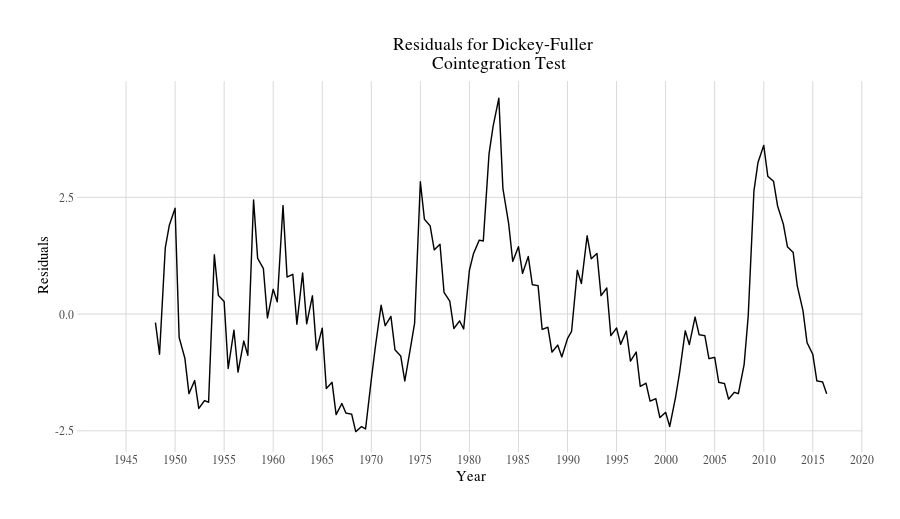
\includegraphics[width=\linewidth]{Resid_DickeyFuller}
	}}
	\medskip\\
	\caption{Residuals for Cointegration Test}
	\label{fig:Resid}
\end{figure}

I conclude that the variables are cointegrated.  Since they are cointegrated, the non-stationarity is actually representative of their relationship and first-differencing the variables would cause bias. There is little theory to support this assumption of cointegration. However, it is important to note that entrepreneurship is poorly understood and the major macroeconomic models essentially ignore it. In other words, assuming that there is a long-run relationship between these two variables, we should reasonably expect there to be very little literature on it, since the literature on entrepreneurship is sparse, contradictory, and inconclusive. Because these variables appear to be cointegrated, the non-stationarity of the data is not a problem. Taking the natural log of the variables makes interpretation of the impulse responses more straightforward, so I run my model in log-levels. 

Although there is reason to believe that my variables are cointegrated, I do not have an especially high level of confidence in that assessment. The theory supporting this assumption is weak, and the tests that pointed towards that conclusion were only marginally significant. Further testing of this assumption could be a fruitful area for future research.

Related to the assumption of cointegration is my decision to use a natural-log transformation on my variables. This transformation allows a convenient interpretation of impulse responses: the percent change in the response variable from trend due to the shock. It's not clear how robust my results are to this assumption. Again, this is a question that future researchers may want to consider.


\subsection{Final Model}

For my final model, I chose a lag length of fourteen years and used biannual data, so I have twenty-eight lags in my model. My main consideration, after performing the analysis shown above, was remaining consistent with the literature's usual lag-order length of eight to fourteen years. Within the constraint of the literature's time-frame, more hypotheses were found to be significant with a lag-order length of fourteen years. I tried to avoid finer granularities because I knew that I intended to use a longer lag-order length and I was concerned that high granularity would result in a model with too many parameters for my data set. This would result in high uncertainty and lots of noise around model estimates and predictions. With months and even quarterly granularities, covering the lag-order length that the literature suggest would necessitate a huge number of parameters. Monthly data with fourteeen years of lags would demand roughly 336 variables in each equation, which is obviously an unsatisfactory model when there are roughly 800 data points per variable. I found that using biannual data with a fourteen year lag-order length resulted in a model that minimized the ratio of estimated coefficients to data points while still finding support for most of my hypotheses. I used log-transformed data in order to simplify interpretation of impulse response functions. In the Model Selection section, I will discuss these choices in more detail.


\section{Results}

The structural model must be translated into a reduced-form model after identification in order to estimate it using maximum-likelihood estimation. I estimated the reduced-form coefficients of my equation using Stata, which recovers the structural equation internally in order to run IRFs, so there was no need to manually recover the structural coefficients. The reduced-form coefficients can be found in Table 3, below. The leftmost column denotes the number of periods (half-years) that the variable is lagged for a given row of coefficients. There are two equations in the model, unemployment. and self-employment--- equations one and two, respectively, in Table \ref{regresults}. Each equation is estimated using lagged values for both variables. The coefficients on each variable for each lag are divided into two subcolumns, sorted by lag value. Again, this is the reduced-form model, not the structural model--- the coefficients for the structural model are not included in this paper.

	\begin{center}
	\begin{longtable}{ccccc}
		\caption{Regression Results}
		\label{regresults} \\
		\hline \hline 
		\textbf{} & \multicolumn{2}{c}{(1) ln(unemp)} & \multicolumn{2}{c}{(2) ln(self-emp)}\\[1mm]
		\hline
		\textbf{Variable: } & \textbf{ln(unemp)} & \textbf{ln(self-emp)} & \textbf{ln(Unemployment}& \textbf{ln(self-emp)} \\
		\endfirsthead
		\multicolumn{4}{c}%
		{\tablename\ \thetable\ -- \textit{Continued from previous page}} \\
		\hline
		\textbf{} & \multicolumn{2}{c}{(1) ln(unemp)} & \multicolumn{2}{c}{(2) ln(self-emp)}\\[1mm]
		\hline
		\textbf{Variable: } & \textbf{ln(unemp)} & \textbf{ln(self-emp)} & \textbf{ln(unemp)}& \textbf{ln(self-emp)} \\
		\hline
		\endhead
		\hline \multicolumn{4}{r}{\textit{Continued on next page}} \\
		\endfoot
		\hline\hline
		\endlastfoot
		\hline
		
		Lag 1        & 1.522***  & 0.514     & 0.023    & 0.699***  \\
		& -0.0925   & -0.331    & -0.0267  & -0.0956   \\
		L2           & -0.620*** & 0.314     & -0.0123  & 0.502***  \\
		& -0.163    & -0.405    & -0.0471  & -0.117    \\
		L3           & -0.228    & -0.956**  & -0.00952 & -0.0733   \\
		& -0.17     & -0.44     & -0.0491  & -0.127    \\
		L4           & 0.421**   & 0.347     & 0.0396   & -0.149    \\
		& -0.17     & -0.426    & -0.0492  & -0.123    \\
		L5           & -0.477*** & 0.553     & -0.037   & 0.0159    \\
		& -0.17     & -0.428    & -0.0492  & -0.124    \\
		L6           & 0.255     & -1.057**  & -0.025   & 0.12      \\
		& -0.166    & -0.431    & -0.048   & -0.125    \\
		L7           & -0.0566   & -0.103    & 0.0353   & -0.189    \\
		& -0.166    & -0.438    & -0.0481  & -0.126    \\
		L8           & 0.0466    & 0.568     & -0.00243 & -0.048    \\
		& -0.154    & -0.428    & -0.0446  & -0.124    \\
		L9           & -0.0871   & 0.257     & -0.0274  & 0.0923    \\
		& -0.142    & -0.444    & -0.0409  & -0.128    \\
		L10          & 0.164     & -0.281    & 0.0308   & 0.00744   \\
		& -0.136    & -0.446    & -0.0392  & -0.129    \\
		L11          & -0.242*   & 0.587     & 0.0183   & 0.0127    \\
		& -0.137    & -0.445    & -0.0397  & -0.129    \\
		L12          & 0.102     & -0.689    & -0.0415  & 0.0833    \\
		& -0.139    & -0.426    & -0.0403  & -0.123    \\
		L13          & -0.0163   & 0.337     & -0.0152  & -0.0772   \\
		& -0.137    & -0.411    & -0.0396  & -0.119    \\
		L14          & 0.0928    & -1.373*** & 0.0854** & -0.19     \\
		& -0.133    & -0.41     & -0.0385  & -0.118    \\
		L15          & -0.0199   & 0.608     & -0.0659* & -0.0522   \\
		& -0.134    & -0.429    & -0.0387  & -0.124    \\
		L16          & -0.067    & 0.419     & 0.0900** & 0.0755    \\
		& -0.133    & -0.422    & -0.0383  & -0.122    \\
		L17          & -0.0661   & 0.422     & -0.0699* & 0.196     \\
		& -0.13     & -0.416    & -0.0374  & -0.12     \\
		L18          & 0.16      & -0.176    & -0.0405  & 0.0425    \\
		& -0.126    & -0.414    & -0.0365  & -0.12     \\
		L19          & -0.0659   & -1.460*** & 0.0521   & -0.074    \\
		& -0.122    & -0.413    & -0.0353  & -0.119    \\
		L20          & 0.188     & 1.274***  & -0.027   & 0.0466    \\
		& -0.122    & -0.426    & -0.0352  & -0.123    \\
		L21          & -0.273**  & 0.209     & 0.0855** & -0.159    \\
		& -0.118    & -0.446    & -0.0342  & -0.129    \\
		L22          & 0.214*    & -1.010**  & -0.053   & -0.00657  \\
		& -0.113    & -0.434    & -0.0325  & -0.125    \\
		L23          & -0.157    & 0.555     & 0.022    & 0.0488    \\
		& -0.112    & -0.426    & -0.0324  & -0.123    \\
		L24          & 0.0183    & -0.299    & -0.0109  & 0.0555    \\
		& -0.108    & -0.421    & -0.0312  & -0.122    \\
		L25          & 0.133     & 0.101     & 0.0184   & -0.347*** \\
		& -0.107    & -0.415    & -0.0308  & -0.12     \\
		L26          & -0.238**  & 0.485     & -0.0248  & 0.127     \\
		& -0.107    & -0.44     & -0.0309  & -0.127    \\
		L27          & 0.156     & -0.252    & 0.0033   & 0.154     \\
		& -0.102    & -0.43     & -0.0295  & -0.124    \\
		L28          & -0.0679   & 0.0553    & 0.0123   & 0.0584    \\
		& -0.0616   & -0.333    & -0.0178  & -0.0962   \\
		& & & & \\
		\textbf{Constant} & \multicolumn{2}{c}{0.493***}  & \multicolumn{2}{c}{-0.0454}    \\
		\textbf{} & \multicolumn{2}{c}{-0.159}  & \multicolumn{2}{c}{-0.046}       \\
		&           &           &          &           \\
		\textbf{Observations} & \multicolumn{2}{c}{110}  & \multicolumn{2}{c}{110}           
		
	\end{longtable}
\end{center}

As discussed above, my hypotheses involve the impulse response functions and Granger-causality tests produced by this model. Impulse response functions (IRFs) have a slightly complicated interpretation, so I will lay it out precisely here, and use more general language for the rest of the section. An impulse response function shows the response of one variable (the response variable) when another variable is shocked (the impulse variable). The shock is produced by increasing (or decreasing) the error term on the equation predicting the impulse variable for one period, after which it returns to zero. Then, the actual response function is derived by finding the difference between the predicted path of the response variable with the shock and the predicted path of the response variable without the shock. So, rather than producing a forecast for the response variable, the reported values are just the part of the response variable's movement that results directly from a shock to the impulse variable.

\subsection{Impulse response: Unemployment on Self-Employment}

My hypothesis about the response of self-employment to unemployment is that a positive shock to unemployment has a positive short-term effect on self-employment. This hypothesis is not supported by the model. I define "short-term" as within five years of the shock. Looking at Figure \ref{fig:IRF_US}, the lower bound of the confidence band does not rise above zero at any point in the first five years after the shock. All predicted values within that time frame are positive, but no value is significantly greater than zero. The graph below shows the impulse response of self-employment to a 1\% shock to unemployment. To be precise, this graph shows the percent difference in the predicted self-employment rate with the shock from the predicted non-shock path of the self-employment rate.

\begin{figure}[!h]
	\centering
	\fbox{\parbox{\textwidth}{\centering
			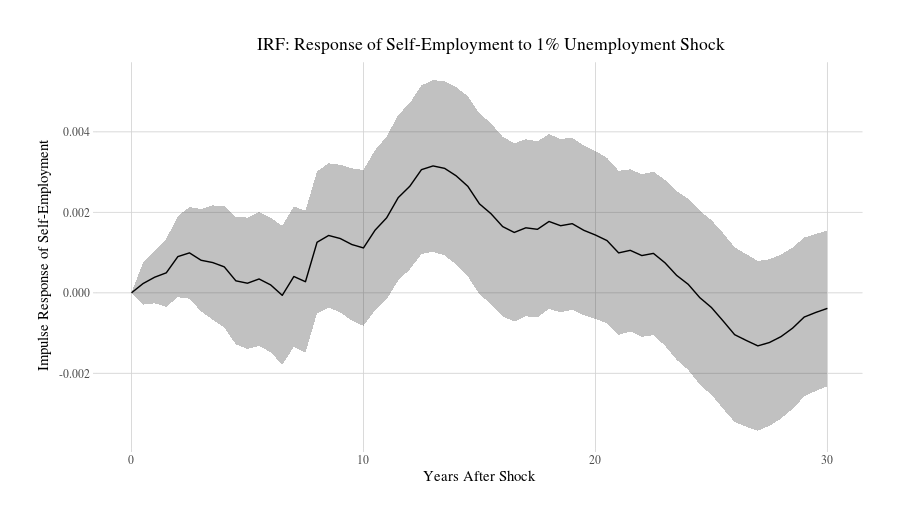
\includegraphics[width=\linewidth]{IRF_US}
	}}
	\medskip\\
	\caption{IRF: Response of Self-Employment Rate to a 1\% Shock in Unemployment }
	\label{fig:IRF_US}
\end{figure}

If there was a significant increase in self-employment between year zero and year five, that finding would support my hypothesis that an increase in unemployment creates a push effect towards self-employment in the short-term. However, if the change in self-employment is not significantly greater than zero at any point during this time range, the model would not provide support for my hypothesis. I will perform formal hypothesis tests in order to determine whether the model supports this hypothesis. First, I will show an example test, and for the rest of the results, you can refer to Table \ref{table:IRF_US}, which gives the test results for all relevant periods. If the t-statistic is greater than 2 or less than -2, then we reject the null; otherwise we fail to reject the null. 

\begin{center}
	\emph{Hypothesis Test:} \\
$H_0$: IRF(1) = 0;  $H_A$ IRF(1) $\neq$ 0 \\
t-statistic = $\frac{\hat{x}}{SE(x)} =\frac{0.001094}{0.001272}=0.860$ \\ 
\end{center} 


\begin{center}
	\begin{longtable}{cccc}
		\caption{Hypothesis Tests for IRF of Unemployment on Self-Employment}
		\label{table:IRF_US} \\
		\hline
		\textbf{Period} & \textbf{$\hat{x}$}  & \textbf{$\hat{SE}(x)$}    & \textbf{Test Statistic} \\
		\hline
		\endfirsthead
		\multicolumn{4}{c}%
		{\tablename\ \thetable\ -- \textit{Continued from previous page}} \\
		\hline
		\textbf{Period} & \textbf{$\hat{x}$}  & \textbf{$ \hat{SE}(x)$}    & \textbf{Test Statistic} \\
		\hline
		\endhead
		\hline \multicolumn{4}{r}{\textit{Continued on next page}} \\
		\endfoot
		\hline
		\endlastfoot
1      & 0.001094            & 0.001272 & 0.860062893    \\
2      & 0.001844            & 0.001573 & 1.172282263    \\
3      & 0.002362            & 0.002048 & 1.153320313    \\
4      & 0.00428             & 0.002446 & 1.749795585    \\
5      & 0.004719            & 0.002763 & 1.707926167    \\
6      & 0.003847            & 0.003084 & 1.247405966    \\
7      & 0.003576            & 0.003444 & 1.038327526    \\
8      & 0.003066            & 0.003659 & 0.837933862    \\
9      & 0.001416            & 0.003836 & 0.369134515    \\
10     & 0.001133            & 0.00396  & 0.286111111   
	\end{longtable}
\end{center}


None of these test statistics are greater than two, so I fail to reject the null hypothesis that self-employment differs from zero for any time period between periods one and ten. I fail to find support for my hypothesis that there is a short-term positive effect of a shock to unemployment on self-employment. Interestingly, there does seem to be a long-term effect. Between IRF(23) and IRF(29), inclusive, which is 11.5 to 14.5  years after the shock, change in self-employment is significantly greater than zero. I did not hypothesize this effect, and I will discuss the implications of this observation in the discussion section.

Given the results in my Model Selection section (see Figure \ref{fig:hm-IRF_US}), I do not believe that my failure to find evidence of a short-term increase in self-employment in response to a shock to unemployment is actually much of an indication about whether or not this effect exists. Figure \ref{fig:hm-IRF_US} implies that my model would not be able to pick up on such an effect if it did exist, because models with lag-order lengths above ten years did not seem sensitive to this effect. A large proportion of the tested models did find evidence for this effect, so perhaps the findings of my final model are not an accurate measure of this effect.

\subsection{Impulse Response: Self-Employment on Unemployment}

The graph below shows the impulse response of unemployment to a 1\% shock to self-employment. The exact interpretation of the graph is the percent difference in the unemployment rate from the predicted non-shock path of the unemployment rate, due to the shock.

\begin{figure}[!h]
	\centering
	\fbox{\parbox{\textwidth}{\centering
			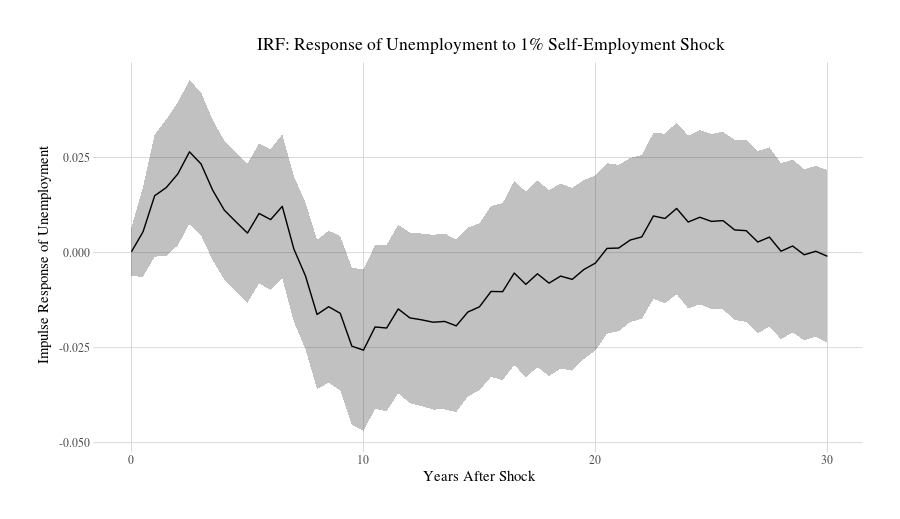
\includegraphics[width=\linewidth]{IRF_SU}
	}}
	\medskip\\
	\caption{IRF: Response of Unemployment Rate to a 1\% Shock in Self-Employment }
	\label{fig:IRF_SU}
\end{figure}

My hypothesis about the response of unemployment to a positive shock on self-employment is that there is a short-term increase in unemployment and a long-term decrease. There appears to be a significant increase in the change in unemployment during periods four to six (year two to the first half of year three), and a significant decrease in periods nineteen and twenty (the second half of year nine and the first half of year ten). Once again, I will give an example t-test and then present a table of the results (see Table \ref{table:IRF_SU}). If the t-statistic is greater than two or less than -2, then we reject the null, otherwise we fail to reject.

\begin{center}
\emph{Hypothesis Test:}\\
$H_0$: IRF(4) = 0; $H_A$: IRF(4) $\neq$ 0 \\
t-statistic =  $ \frac{\hat{X}}{SE(X)} = \frac{0.028456}{0.013177} = 2.1595$ \\
\end{center}

\begin{center}
	\begin{longtable}{cccc}
		\caption{Hypothesis Tests for IRF of Self-Employment on Unemployment}
		\label{table:IRF_SU} \\
		\hline
		\textbf{Period} & \textbf{$\hat{x}$}  & \textbf{$\hat{SE}(x)$}    & \textbf{Test Statistic} \\
		\hline
		\endfirsthead
		\multicolumn{4}{c}%
		{\tablename\ \thetable\ -- \textit{Continued from previous page}} \\
		\hline
		\textbf{Period} & \textbf{$\hat{x}$}  & \textbf{$ \hat{SE}(x)$}    & \textbf{Test Statistic} \\
		\hline
		\endhead
		\hline \multicolumn{4}{r}{\textit{Continued on next page}} \\
		\endfoot
		\hline
		\endlastfoot
Period & $\hat{x}$  & $ \hat{SE}(x)$    & Test Statistic \\
4      & 0.028456            & 0.013177 & 2.159520376    \\
5      & 0.0364              & 0.013225 & 2.752362949    \\
6      & 0.032022            & 0.013181 & 2.429405963    \\
\hline
19     & -0.033789           & 0.014478 & -2.333816826   \\
20     & -0.035245           & 0.014855 & -2.372601818  
	\end{longtable}
\end{center}


\pagebreak
I reject the null hypothesis for all five tests, clearly demonstrating that there is a significant increase in the growth rate of unemployment in the short-term and a significant decrease in the long-term in response to a positive shock to growth in self-employment . There are no other time periods that significantly differ from zero in this IRF. 

This IRF is also useful in that it provides information about the timing of these responses. The only periods with a predicted value that differs significantly from zero are those detailed above: periods four, five, and six (the second half of the second year following the shock through the end of the third year); and periods nineteen and twenty (the tenth year following the shock). Additionally, between period zero and period fourteen, inclusive, the predicted value for unemployment is always positive. Then, from period fifteen until period forty, it becomes negative. This pattern may offer indications that later studies can look for. In summary, given a positive shock to unemployment, there is likely an increase in unemployment within two years for around a year and a half, and a decrease around the tenth year. There are rough indications that there may be a positive effect for around seven years, which then turns into a negative effect for the next decade. However, this second observation is not statistically significant, so it is merely a speculative indication for future researchers to consider. 

\subsection{Granger-causality}

I had two additional hypotheses about this model: that unemployment would Granger-cause self-employment and that self-employment would Granger-cause unemployment. If one variable Granger-causes another, that means that the first variable is significantly useful in predicting future values of the second variable, in addition to previous values of the predicted variable. Clearly, this is not a test of "causation" as the term is commonly used. However, when combined with solid theory and other evidence, it can provide support for a hypothesis of causation. The null hypothesis for a Granger-causality test is that, compared to the predictive power of the past values of time-series Y on future (within-sample) values of Y, using past values of both X and Y will not add significant predictive power. The alternative is that past values of X do, in fact, add a significant amount of predictive power in addition to past values of Y. I ran a Granger-causality test on both variables, and found that the null hypothesis was rejected at an $\alpha = 0.001$ level in both cases. This indicates that past values of self-employment are useful for predicting values of unemployment, as compared to using only past values of unemployment to predict future value of unemployment; it also indicates the same for the other direction: past values of unemployment are useful for predicting future values of self-employment.

\subsection{Summary of Results and Policy Implications}

I find evidence that self-employment and unemployment rates are useful in predicting future values of each other; I find that a shock to self-employment causes a short-term increase in unemployment two to three years after the shock followed by a long-term decrease ten years after the shock. All but one of my hypotheses were supported by the model. The hypothesis I failed to find support for is that a positive shock to unemployment causes a short-term increase in self-employment as compared to the predicted values of self-employment if there were no shock.

These findings have important implications for policy. Especially if an administration is considering incentivizing entrepreneurship as a response to an economic downturn, it's important to balance the longer-term positive effects on growth with the short-term expected increase in the unemployment rate. It seems to me that the ideal time to stimulate entrepreneurship is during an economic upturn, since shorter-term effects may be a problem in the midst of a recession or a recovery. Real concerns about political stability arise when the unemployment rate rises too high, so making policy that increases the unemployment rate when it's already high may be a mistake. However, it does seem that stimulating entrepreneurship is a positive for employment in the long-term, and the literature certainly indicates that it supports long-term growth in GDP as well, along with innovation and increased market efficiency \cite{matejovsky14, dejardin11}. Hopefully this paper will support policymakers by providing more information about how the economy responds to changes in entrepreneurship.


\section{Model Selection: Lags and Granularity}
\subsection{Overview}
In order to choose lag-length and granularity, I ran a series of models with various combinations of different lag-orders and granularities. I tested the following granularities: monthly, quarterly, half-yearly (biannually), and annually. In this paper, I'll use "lag-order length" to refer to the number of years covered by the lags in a model. So a lag-order length of one year means that the lags of that model, no matter the granularity, span one year. For model using monthly data, a lag-order length of one year means there are twelve lags; for a model using annual data, a lag-order length of one year means there is one lag. I tested a lag-order length of one year, plus all even lag-order lengths between two and fourteen years, inclusive. One additional consideration during this process was model stability. In order to interpret impulse-response functions, there is an extra restriction that must be met: stability. A VAR model is stable "if its reverse characteristic polynomial has no roots in and on the complex unit circle" (Lutkepohl, 16). Models that were unstable were excluded from consideration, since their impulse responses have no interpretation. For every granularity, using more than fourteen years of lags resulted in an unstable model, so no tests used greater than fourteen years of lags. Using monthly data, models with greater than six years of lags were unstable, so there were fewer lag-order lengths tested with monthly data than with the other granularities. For each model, I noted which hypotheses were supported by that model, and used that to create a graphic for each hypothesis, showing which models find support for that hypothesis. The results of this analysis are summarized below using a series of heatmaps. A heatmap is essentially a table with each cell color-coded by its value in order to make patterns more easily visible. Each heatmap shows the level of support for one hypothesis across all tested models. I will briefly discuss each heatmap after presenting it.

\begin{figure}[!h]
	\centering
	\fbox{\parbox{\textwidth}{\centering
			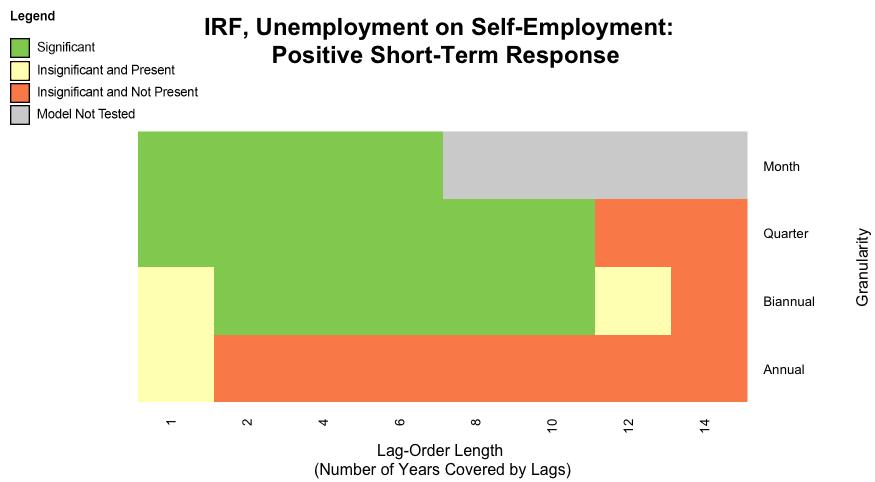
\includegraphics[width=\linewidth]{hm-IRF_US}
	}}
	\medskip\\
	\caption{Heatmap: Response of Unemployment Rate to a 1\% Shock in Self-Employment Across Models}
	\label{fig:hm-IRF_US}
\end{figure}

\subsection{Discussion of IRF, Unemployment on Self-Employment (See Figure \ref{fig:hm-IRF_US})}
This heatmap is the impetus for a major caveat to this paper that I discussed above in the Results section. Although my final model fails to provide evidence that self-employment has a positive short-term response to a shock to unemployment, more than 50\% of the models tested found significant evidence for this effect. Further, it's possible that using a longer lag-order simply reduces the sensitivity of the models enough that this effect is not picked up. If that were true, then we could exclude models with greater than ten years of lags from consideration when seeking evidence for or against this hypothesis. No models with greater than ten years of lags found support for this hypothesis, and 68\% of models (at all granularities) with ten or fewer years of lags found significant support for this hypothesis. So there does seem to be a pattern that models with longer lag-order lengths are less likely to find support.

It also seems that something about annual lags causes models to miss this effect. One explanation is that within-period noise dominates over such a small effect when each period is long enough. In other words, because the effect is short-lived, random variations that occur after the positive response but also within the same measurement period of the shock drown out the small, brief positive response. Shorter time-frames (finer granularities) are able to pick up the effect because a larger share of the other variation that occurs after it is separated into a different period. 

Overall, about half of the tested models find support for this hypothesis. Despite the fact that my final model does not find support for this hypothesis, there is some evidence that it exists.


\begin{figure}[!h]
	\centering
	\fbox{\parbox{\textwidth}{\centering
			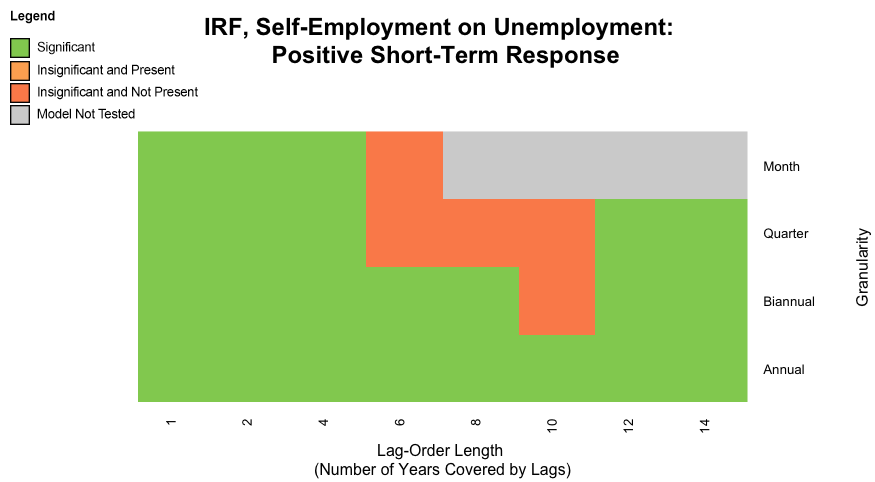
\includegraphics[width=\linewidth]{hm-IRF_SUI}
	}}
	\medskip\\
	\caption{Heatmap: Response of Unemployment Rate to a 1\% Shock in Self-Employment, Long-Term Increase Across Models}
	\label{fig:hm-IRF_SUI}
\end{figure}

\subsection{Discussion of IRF, Self-Employment on Unemployment, Short-Term Effect (See Figure \ref{fig:hm-IRF_SUI})}
My final model found evidence that a shock to self-employment causes a short-term increase in unemployment. Twenty-three of the twenty-eight tested models, or 82\% of them, found significant evidence to support this hypothesis. That is a remarkably high proportion. My findings are very robust to changes in lag-order length and granularity. Interestingly, lags-orders covering 6-10 years seem to be slightly less likely to find evidence for this effect.
 
 \begin{figure}[!h]
 	\centering
 	\fbox{\parbox{\textwidth}{\centering
 			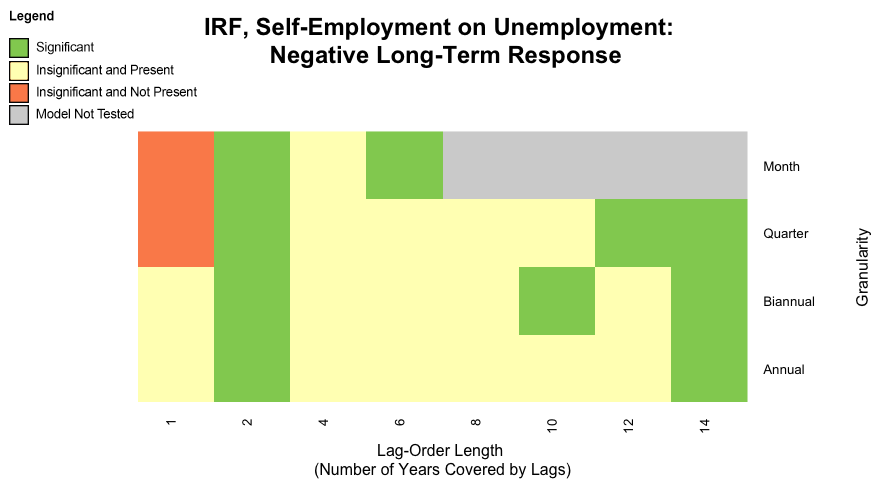
\includegraphics[width=\linewidth]{hm-IRF_SUD}
 	}}
 	\medskip\\
 	\caption{Heatmap: Response of Unemployment Rate to a 1\% Shock in Self-Employment, Short-Term Decrease Across Models}
 	\label{fig:hm-IRF_SUD}
 \end{figure}

 \subsection{Discussion of IRF, Self-Employment on Unemployment, Long-Term Effect (See Figure \ref{fig:hm-IRF_SUD})}
 My final model found evidence that a shock to self-employment causes a long-term decrease in unemployment. Ten of the twenty-eight tested models, or 35\% of them, found significant evidence for this effect. Models with longer lag-orders as well as models with a lag-order covering two years seem to be more likely to find this effect. With a lag-order length of fourteen years (as used in my final model), my findings are robust to granularity of the data. However, they are not robust to changes in lag-order.
 
\begin{figure}[!h]
	\centering
	\fbox{\parbox{\textwidth}{\centering
			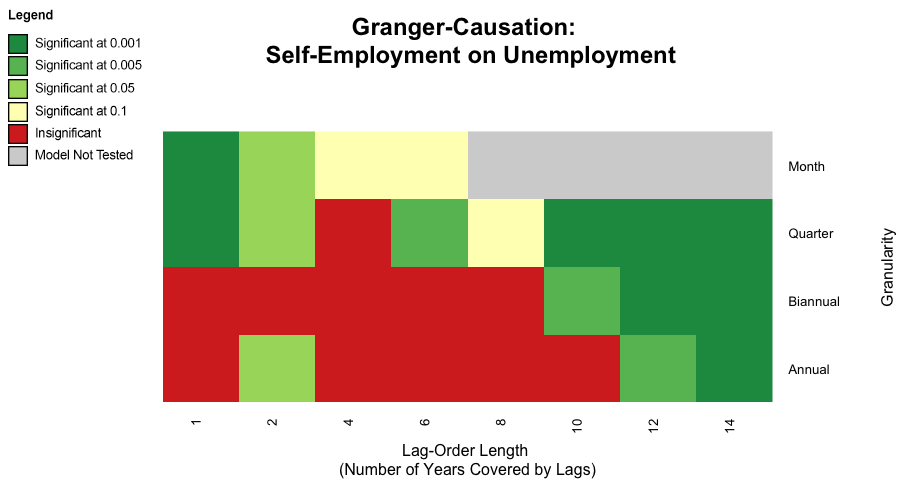
\includegraphics[width=\linewidth]{hm-GC_SU}
	}}
	\medskip\\
	\caption{Heatmap: Granger-Causality of Self-Employment on Unemployment Across Models}
	\label{fig:hm-GC_SU}
\end{figure}
\subsection{Discussion of Granger-Causation, Unemployment on Self-Employment (See Figure \ref{fig:hm-GC_SU})}
Eleven of the twenty-eight tested models, or 39\% of them, found significant evidence that self-employment is an effective predictor of future values of unemployment. Longer lag-orders seem more likely to find evidence of this. That could indicate that it takes several years for self-employment to affect unemployment (perhaps around ten, which is when models start to find significance most of the time). This is unsurprising because it's consistent with both theory and the literature; it takes several years before a new company grows large enough to have a meaningful effect on employment levels. My findings are robust to changes in granularity and somewhat robust to changes in lag-order length.
 
\begin{figure}[!h]
	\centering
	\fbox{\parbox{\textwidth}{\centering
			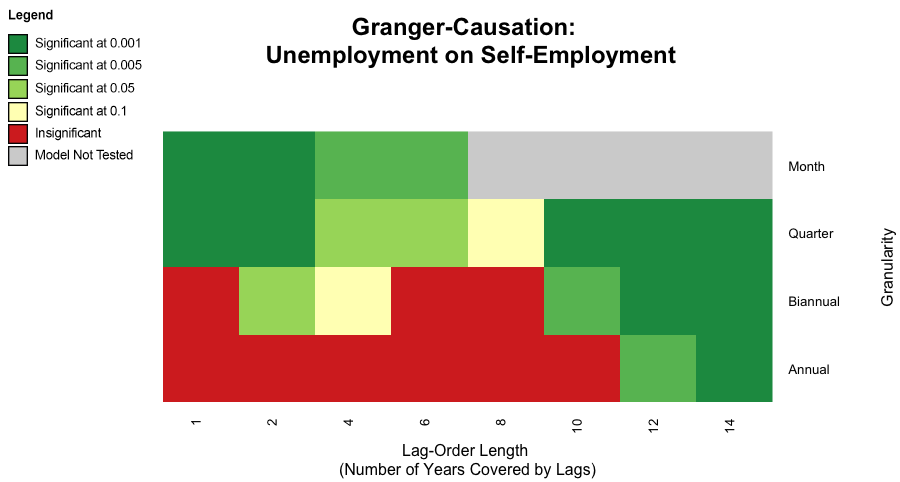
\includegraphics[width=\linewidth]{hm-GC_US}
	}}
	\medskip\\
	\caption{Heatmap: Granger-Causality of Unemployment on Self-Employment Across Models}
	\label{fig:hm-GC_US}
\end{figure}

\subsection{Discussion of Granger-Causation, Self-Employment on Unemployment (See Figure \ref{fig:hm-GC_US})}
Fourteen of the twenty-eight tested models, or 50\% of them, found significant evidence that unemployment is a useful predictor of future values of self-employment. Longer lag-order lengths seem to provide greater sensitivity to this effect, implying that some effects in this direction may take place over a longer period of time. However, finer granularities with short lag-order lengths also seem to support this hypothesis. It may be that there are weak short-term effects and strong long-term effects, so that models with longer lag-order lengths find significance as well as short lag-order lengths using finer granularities. My findings are robust to changes in granularity and somewhat robust to changes in lag-order length.

%\subsection{Summary of Robustness and Model Selection}



\section{Discussion}

\subsection{Unexpected Result in IRF of Self-Employment's Response to a Shock in Unemployment}

I hypothesized that a positive shock to unemployment would cause a short-term increase in self-employment, but I found instead that the only significant effect was a long-term increase, around twelve to fourteen years after the shock. This was unexpected, and there does not seem to be a clear explanation suggested by the relevant theory. It seems likely that there is some third variable that is causing this change. One possible explanation for this is that recessions are interacting with some peculiarity of human psychology to create this lagged effect. Imagine that a major recession hits, unemployment rises, and citizens suddenly feel like their regular employment situations are much more unstable than they had previously realized. As the economy starts to recover and they once again have real opportunities for regular employment and self-employment, they may be more likely to choose self-employment due to their negative experience with regular employment during the recession. This hypothesis may require us to make unusual assumptions, like that people weight their own experiences very heavily--- perhaps more heavily than would be rational. 

This could be an interesting area for future research. Considering other third variables may uncover some other important interaction that causes this effect. If that fails, then perhaps it would be worth considering a psychological/behavioral approach to this problem, in case this turns out to be caused by some sort of common human heuristic or bias. 
	
\subsection{Limitations and Future Research}

One important limiting factor in this study is my use of self-employment as a measure of entrepreneurship. As discussed in the literature review, measuring entrepreneurship is a difficult task, made harder by the loose meaning of the word "entrepreneur." In fact, the theoretical basis for my hypotheses point to several different meanings of the word. When unemployment rises, we expect to see an increase in people who start their own businesses, but not necessarily an increase in innovative (Schumpeterian) entrepreneurs. However, when I hypothesize that an increase in "entrepreneurship" may result in a long-term decrease in unemployment, I am specifically referring to Schumpeterian entrepreneurs. The strongest theory concerning the effect of entrepreneurship on unemployment certainly refers specifically to Schumpeterian entrepreneurship, not just individuals starting their own businesses. It's very difficult to pick apart these intertwined threads, and sometimes it's simply not worth the effort (as, I believe, it isn't worth it in this paper). The division of entrepreneurship into these types is, from a measurement perspective, quite artificial. However, it is worth noting because my choice of measure means that I'm picking out a narrow subset of entrepreneurs with a particular set of traits and expected behaviors. This is not a representative sample out of the pool of all entrepreneurs. Therefore, my results may not generalize well to other types of entrepreneur. 
	
The question of defining different types of entrepreneurship and evaluating the effects of each type individually is an incredibly important topic for future research. One of the major difficulties in the study of entrepreneurship is that, since different researchers are operating from different definitions, they find conflicting results, and the literature becomes scattered and confusing. I focus on self-employment as a measure of entrepreneurship, primarily because it is easy to measure. Self-employment is a subset of entrepreneurship that has low growth-potential, takes on very little capital, and is responsible for a very small share of employment relative to the number of businesses in the category. A follow-up study could use a similar model that targets a similar time frame in the US, but uses a measure that better captures high growth-potential entrepreneurship (e.g. businesses that take on large quantities of venture capital). 

Another interesting area for future studies to investigate is including a measure of growth and/or the business cycle in a model of the entrepreneurship-unemployment relationship. The literature indicates that GDP growth may be an important mediating factor in this relationship. The idea that entrepreneurial activity results in innovation, which results in growth (and which, in turn, decreases unemployment) is firmly fixed in the popular mind of the US. This hypothesis may be true, but there is enormous uncertainty around the actual mechanics of this causal chain. In addition, it's unclear exactly why entrepreneurship seems to be a vehicle for innovation (while there are some popular hypotheses, the evidence is weak). 	

I considered including GDP or GDP growth in my model, both endogenously and exogenously.  However, I found that my models were improved by excluding GDP and its variants altogether. Neither exogenous GDP nor exogenous GDP growth were significant at an $\alpha = 0.05$ level. Including GDP or GDP growth endogenously created excessive uncertainty in the IRFs and resulted in unstable models. When including enough lags to capture the long-term effects of self-employment on unemployment as well as endogenous GDP, the confidence intervals around IRFs became too large and, despite large predicted effects, none were significant. Further, models became unstable with lag-lengths of greater than nine years. Therefore, GDP was not included in my model.

I suspect that one weakness of this study is the simplicity of my model selection process. Even though I am using an unusually large dataset compared to the literature on this topic, I still found clear signs that, as I approached a lag-order that sufficiently captured this relationship, the sensitivity of the model dropped off enough to make it essentially useless. This is clearly highlighted in the Model Selection section (se Figures \ref{fig:hm-IRF_US} to \ref{fig:hm-GC_US}). A study using a sparse VAR (i.e. a VAR with constraints placed on those coefficients that are deemed unnecessary) would have greater statistical power and still be able to uncover the effects that appear with larger lag-orders \citep{sparse}. While many features of the conventional reduced-form VAR are uniquely appropriate for studying this research question, a more parsimonious model could have a large advantage over a conventional VAR, especially considering my findings from the Model Selection section, which indicate that the model may have lost the statistical power to discern one of the hypothesized effects due to inclusion of a large number of estimated coefficients.

\section{Conclusion}

In this study, I used a large and high-frequency dataset to investigate the relationship between entrepreneurship and unemployment in the US. Entrepreneurship is generally seen as an unequivocal good in the U.S., and policy is often enacted based up on this premise. However, the actual, concrete effects of entrepreneurship on the economy are poorly understood. As a recent example, Obama's administration has enacted many policies to support entrepreneurs with a clear expectation that doing so will raise the employment level and "create prosperity" \citep{obama}. There is certainly reason to believe that reducing barriers to entrepreneurship has a positive effect on the economy (Gries 2009). However, there is also evidence that increases in entrepreneurship can significantly increase unemployment in the short term, with negative effects on employment lasting for several years. Such effects would be very important to consider when enacting policy that encourages entrepreneurship while the country is in the midst of a recession. My study aims to refine expectations about the way unemployment responds to entrepreneurship (and vice versa) in the U.S. economy. 

I find that a positive shock to entrepreneurship causes an increase in unemployment two and three years after the shock and a decrease in unemployment in the tenth year after the shock. Further, these two variables are important predictors (and probably causal influences) on each other. These findings are consistent with the literature and contribute important evidence towards this area of research. My final model also fails to find support for a hypothesis that is supported by several other papers: that a shock to unemployment will cause a short-term increase in self-employment. Although my final model does not support this hypothesis, results from my model-selection process indicate that a more sensitive model would likely have found evidence for this effect.

There are several areas of future research pointed to by my findings in this study. Firstly, building a more-sensitive model, possibly using a sparse VAR, would be a large step forwards. There are several effects here, taking place over a long period of time, and it is challenging to select a model that is sensitive to the effects that are of a smaller scale while spanning a long-enough period of time to pick up the long-term effects. Secondly, the role of GDP in this relationship is an interesting area of investigation. Past literature and theory both suggest that it plays an important role in mediating this relationship, but the scale and time-span of my project did not allow me to overcome the challenges involved in incorporating GDP effectively into this model. Thirdly, and perhaps most importantly, there is much work to be done in understanding and defining the roles and differing effects of the many subsets of "entrepreneurship." This study investigated one particular group of entrepreneurs, but the self-employed are not an especially high growth-potential group of entrepreneurs, and other types of entrepreneur may have differing effects on (and be affected differently by) unemployment.

In summary, unemployment and entrepreneurship have significant effects on each other, and policymakers need to be conscious of those effects when manipulating the incentives for entrepreneurship as a policy lever. After a shock to entrepreneurship, there are short-term positive effects and long-term negative effects on unemployment. Therefore, encouraging entrepreneurship may not be a useful policy tool during and immediately after recessions.

\section*{Acknowledgements}

Many thanks to Stephie Fried for her support and guidance during this project. She is a dedicated and supportive professor, and I'm grateful to have had her as my advisor.



\bibliographystyle{ecca}
\bibliography{Bibliography1.bib}

\end{document}
